Variables related to the $B$-meson direction (or simply -- angular observables) can provide a strong separation between $\BB$ decays and $\qqbar$ jets.
It can be understood from the point of view, that a spinless \FourS decaying into two \B mesons will result in a $1-\cos^2\theta_B$ distribution with respect to the $z$ axis.
On the other hand, half-integer spin $\epem\ra\qqbar$ decays follow a $1+\cos\theta_B^2$ distribution \cite{BaBar:2014omp}.
Six variables are tested in this analysis:
\begin{itemize}
    \item $\theta_B$: the momentum angle of the $B$ meson;
    \item $\Delta\theta_B$: the uncertainty of $\theta_B$;
    \item $\theta_{B\wedge B_n}$: the angle between the $B$ meson momentum, and the nominal-$B$ angle calculated using beam-energy constraints;
    \item $\theta_{B\wedge XY}$: the angle between the $B$ meson momentum and the vertex vector in the $xy$-plane;
    \item $\theta_{B\wedge V}$: the angle between the $B$ meson momentum and the vertex vector,
    \item $\theta_{B\wedge T}$: the angle between the $B$ meson momentum and the thrust vector $\vec{T}$.
\end{itemize}
The results for \textbf{Test~1} are given in \Cref{fig:Btag_cosTheta,fig:Btag_cosThetaErr,fig:Btag_cosThetaBetweenParticleAndNominalB,fig:Btag_cosAngleBetweenMomentumAndVertexVectorInXYPlane,fig:Btag_cosAngleBetweenMomentumAndVertexVector,fig:Btag_cosToThrustOfEvent}.
As many angular variables are used in \FEI training, these variables turned out have strongly biased \Mbc distributions.

\begin{figure}[htbp!]
    \subcaptionbox{\label{fig:Btag_cosTheta}}{
        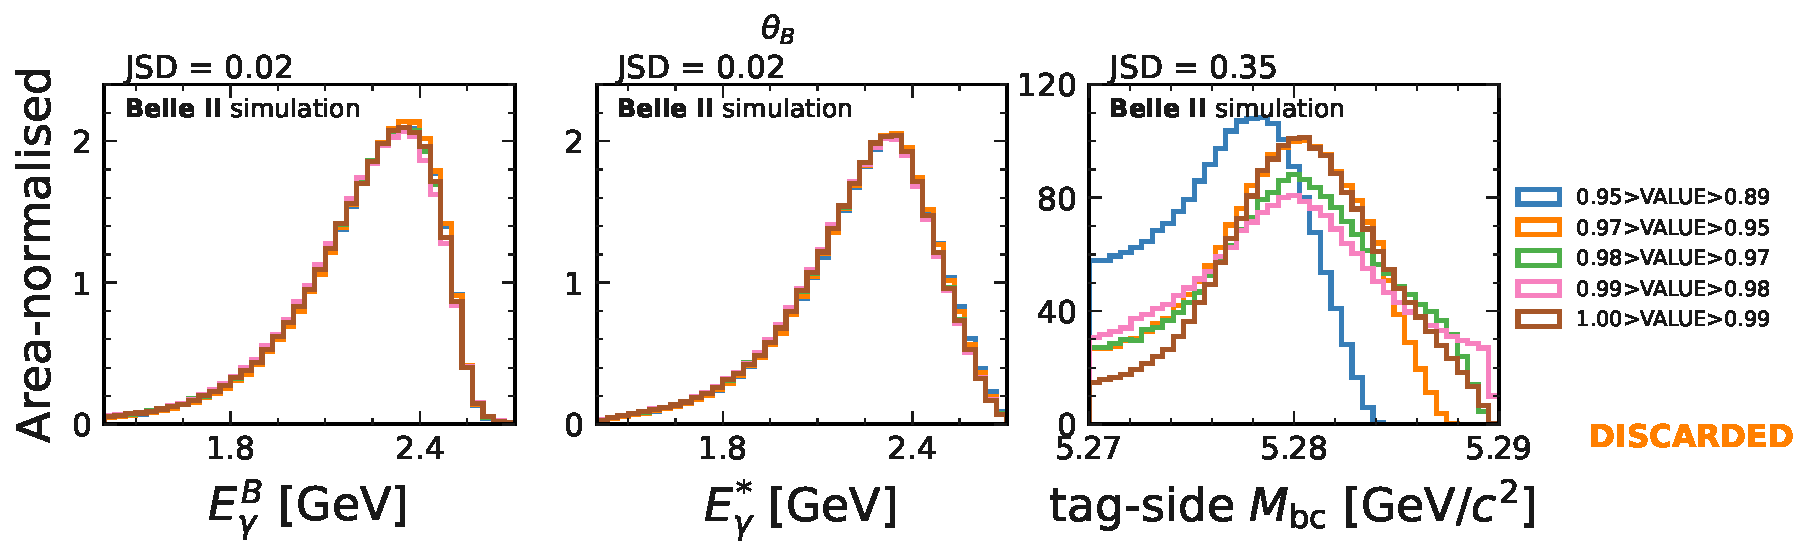
\includegraphics[width=1\textwidth]{figures/appendices/continuum_suppression_features/angular_features/Btag_cosTheta_bias_tested.pdf}
    }
    \subcaptionbox{\label{fig:Btag_cosThetaErr}}{
        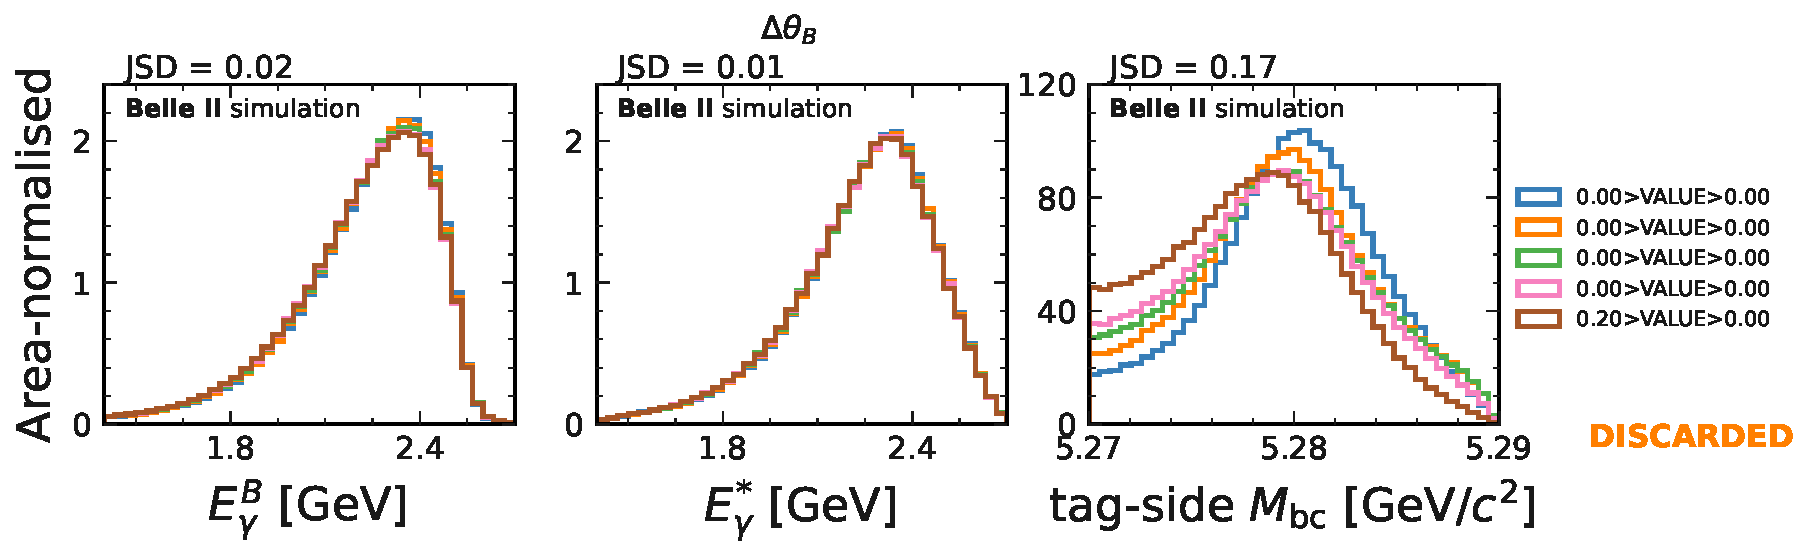
\includegraphics[width=1\textwidth]{figures/appendices/continuum_suppression_features/angular_features/Btag_cosThetaErr_bias_tested.pdf}

    }
    \subcaptionbox{\label{fig:Btag_cosThetaBetweenParticleAndNominalB}}{
        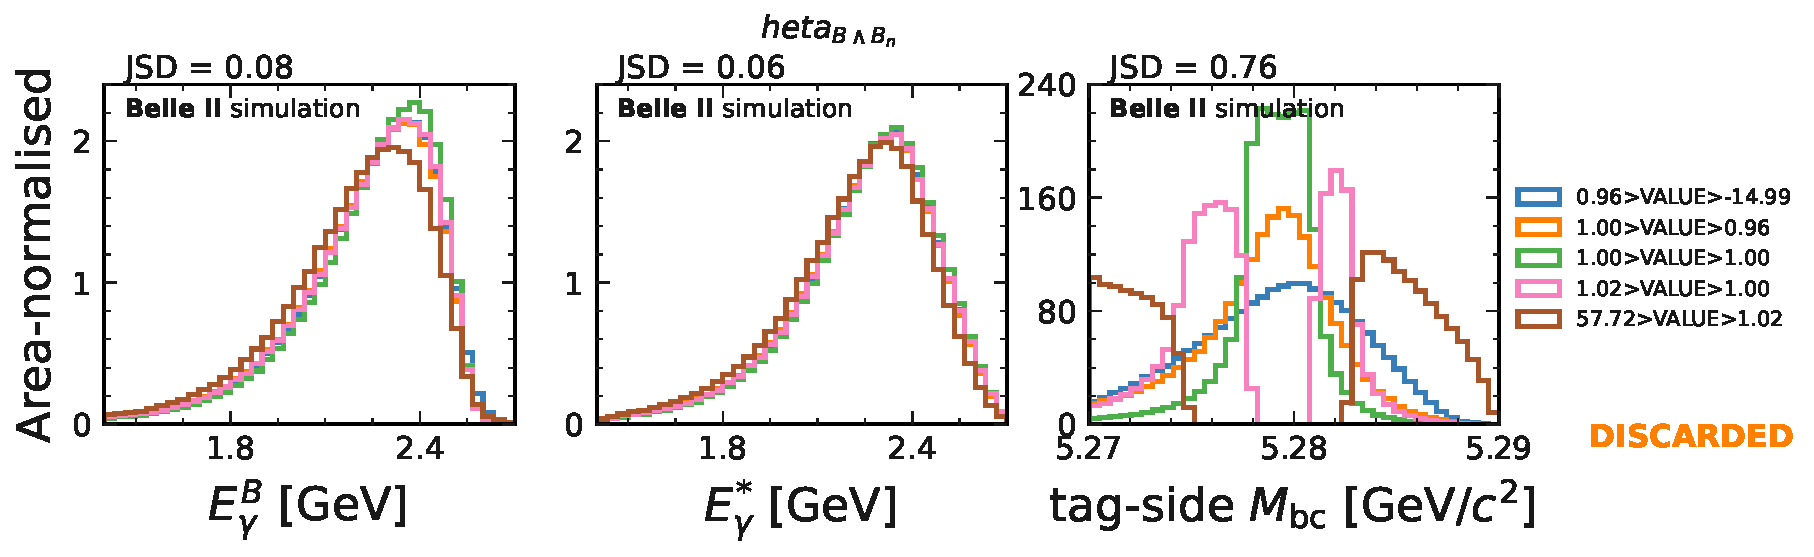
\includegraphics[width=1\textwidth]{figures/appendices/continuum_suppression_features/angular_features/Btag_cosThetaBetweenParticleAndNominalB_bias_tested.pdf}

    }
\end{figure}
\begin{figure}[htbp!]
    \ContinuedFloat

    \subcaptionbox{\label{fig:Btag_cosAngleBetweenMomentumAndVertexVectorInXYPlane}}{
        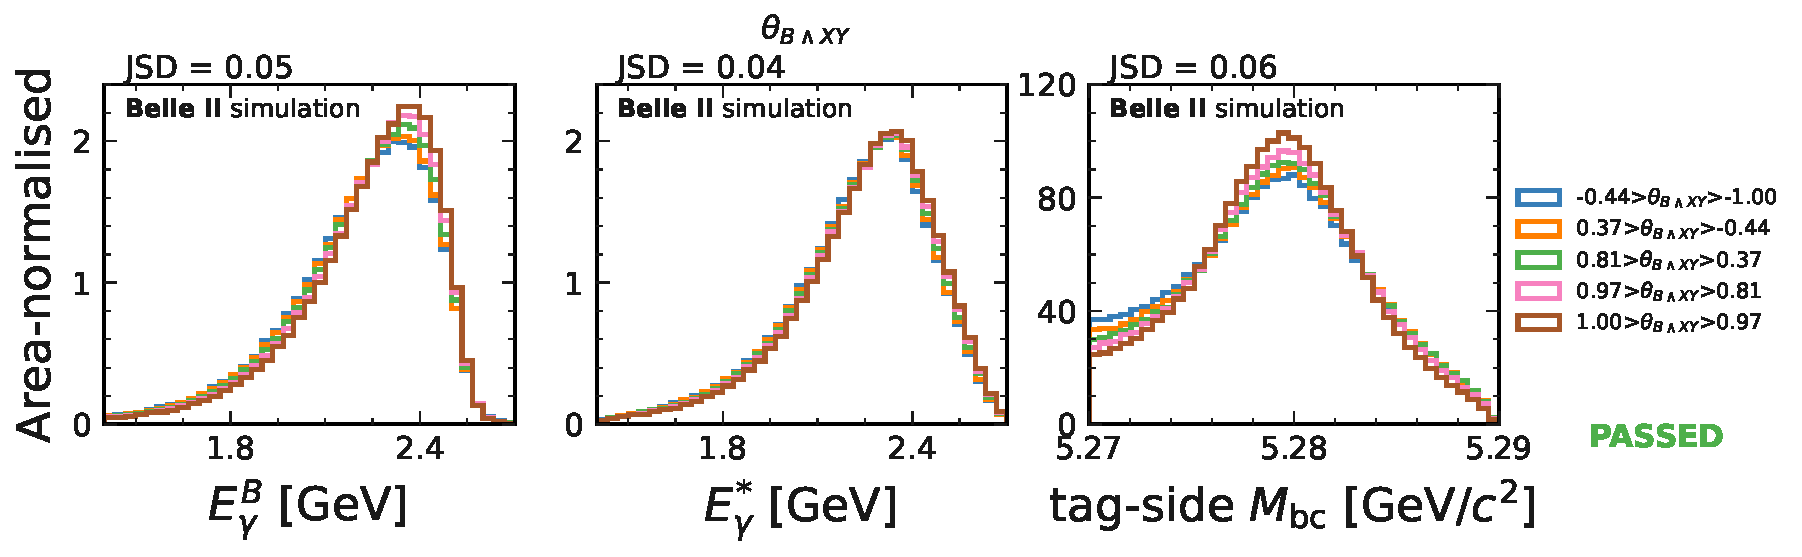
\includegraphics[width=1\textwidth]{figures/appendices/continuum_suppression_features/angular_features/Btag_cosAngleBetweenMomentumAndVertexVectorInXYPlane_bias_tested.pdf}

    }
    \subcaptionbox{\label{fig:Btag_cosAngleBetweenMomentumAndVertexVector}}{
        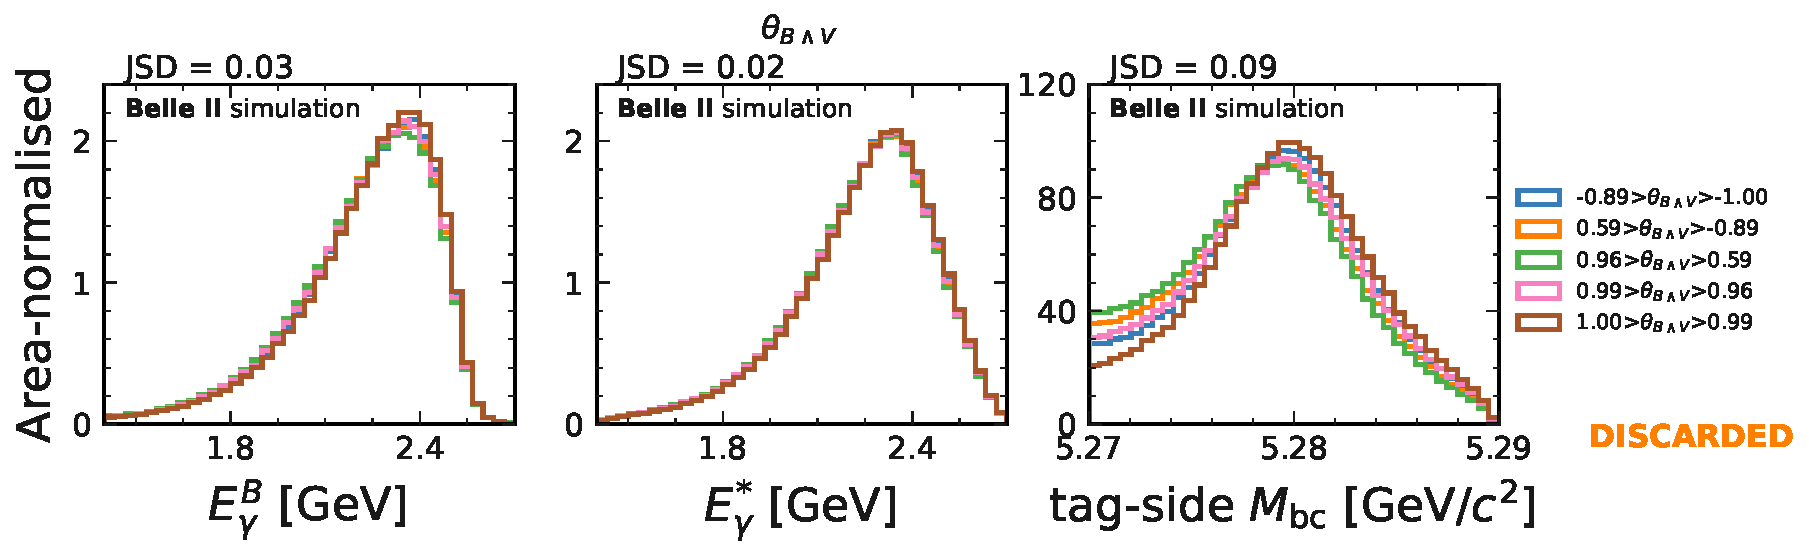
\includegraphics[width=1\textwidth]{figures/appendices/continuum_suppression_features/angular_features/Btag_cosAngleBetweenMomentumAndVertexVector_bias_tested.pdf}

    }
    \subcaptionbox{\label{fig:Btag_cosToThrustOfEvent}}{
        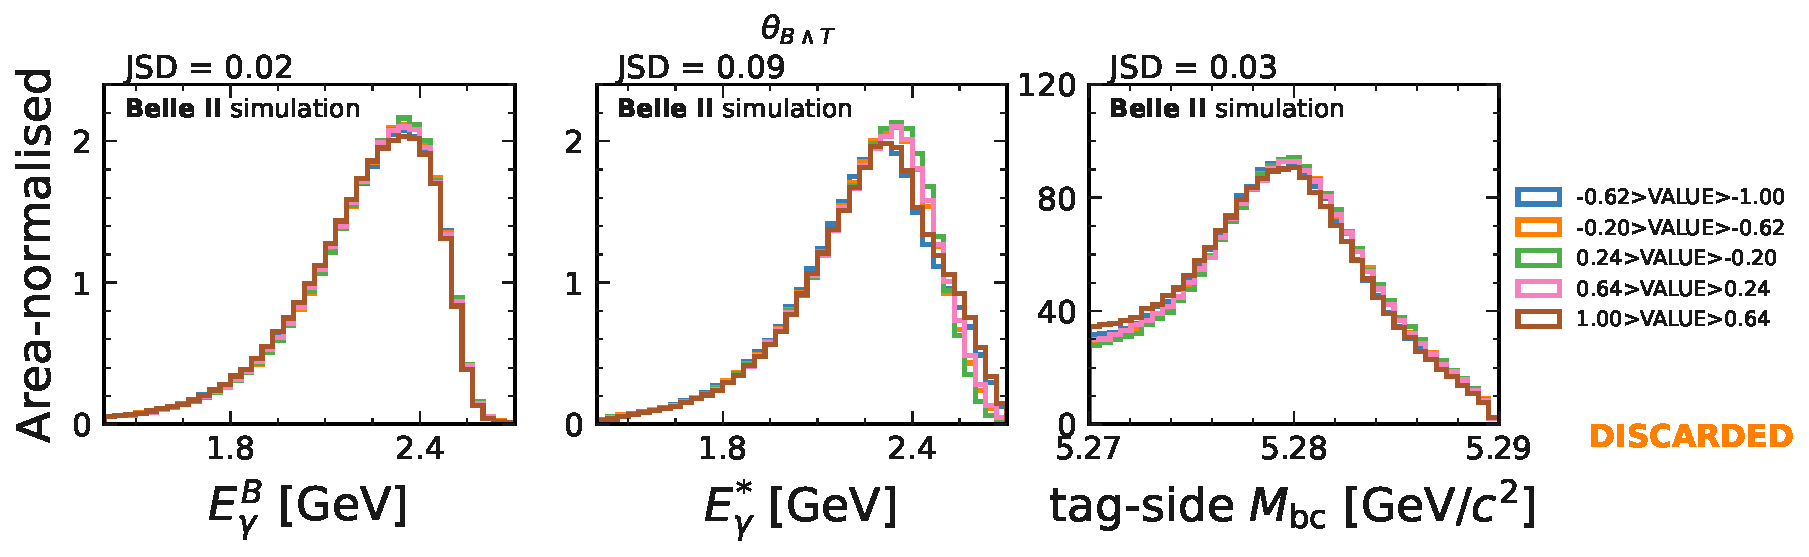
\includegraphics[width=1\textwidth]{figures/appendices/continuum_suppression_features/angular_features/Btag_cosToThrustOfEvent_bias_tested.pdf}

    }
    \caption{\label{fig:angular_features_test1} The bias-test on \EB, \Estar and \Mbc for angular observables of the $B$ meson.
    The test is performed based on \textbf{Test~1} strategy, defined in \Cref{sec:continuum_features}.
    Variable definitions are given in text.}
\end{figure}